\begin{document}
	\chapter{Results}
	
	The study conducted over the data gathered served for the definition of new metrics to measure the performance and robustness of the Lightning Network and for the formal modeling of two mathematical representation of the Lightning Network, from a static and dynamic point of view. The analysis is carried over a period of one month, one snapshot per day; this observation period will be justified by the results obtained by the analysis of daily behavior of the network that will be shown next. 
	
	\section{Trends}
	
	The following section takes in consideration the most relevant trends of the network which are the nodes and edges variation, the average degree and the diameter of the network on a daily and a monthly basis. The analysis carried over the daily basis data is made to justify the decision of the focus on a larger time window. The reasons behind the following churn rates are out of the scope of this work, but it is likely that they largely depends on protocol changes, client errors and, possibly the popularity of the network itself.
	
	A full day representation of the Lightning Network consists of 144 snapshots taken at 10 minutes intervals; the 10 minutes intervals were chosen because every channel that is added (or removed) from the network must wait for the funding transaction (settlement transaction in case a channel is being closed) to be included in a block and added to the chain by the miners. The following results matched the expectation because, as stated in the white paper, a Lightning node and its channels are meant to have a long lifespan. The data refers to the date of 16th of May, 21th of May ,26th of May, 2nd of June, 
	
	\subsection{Daily nodes variation}
	
	\begin{figure}[h]
		\centering
		\begin{subfigure}{0.45\textwidth}
			\centering
			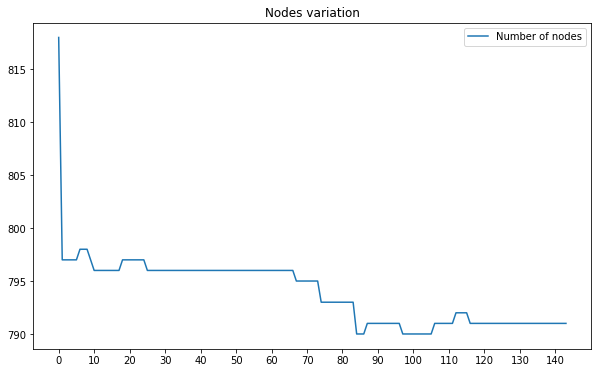
\includegraphics[width=\linewidth]{daily_number_of_nodes0}
			\caption{Snapshot, May 16th}
			\label{daily_node0}
		\end{subfigure}
		\begin{subfigure}{0.45\textwidth}
			\centering
			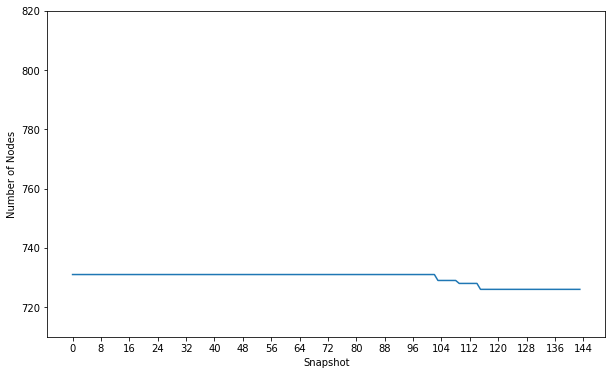
\includegraphics[width=\linewidth]{daily_number_of_nodes1}
			\caption{Snapshot, May 21th}
			\label{daily_node1}
		\end{subfigure}
			\begin{subfigure}{0.45\textwidth}
			\centering
			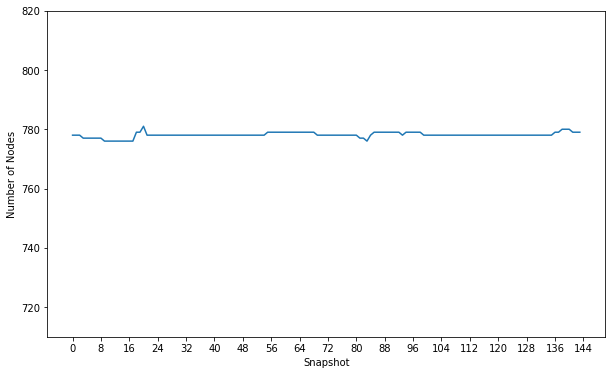
\includegraphics[width=\linewidth]{daily_number_of_nodes2}
			\caption{Snapshot, May 26th}
			\label{daily_node2}
		\end{subfigure}
		\begin{subfigure}{0.45\textwidth}
			\centering
			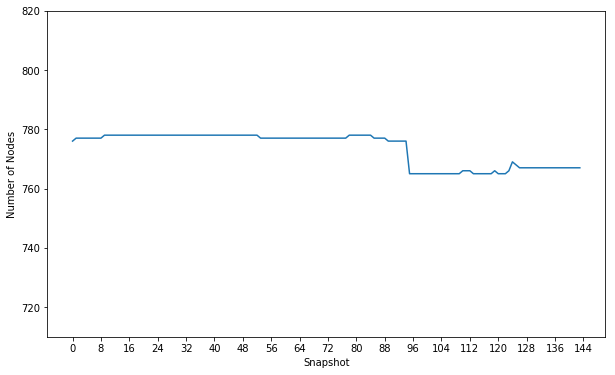
\includegraphics[width=\linewidth]{daily_number_of_nodes3}
			\caption{Snapshot, June 2nd}
			\label{daily_node3}
		\end{subfigure}
		
		\caption{Nodes trends on a daily basis}
		\label{daily_nodes_variation}
	\end{figure}

	Details on nodes variations on a daily basis are reported in \ref{daily_nodes_variation}. The figure shows the 144 snapshot of the network for four different days. We can notice a similar behavior between the snapshots pictured in (\ref{daily_node1}) and (\ref{daily_node3}), although we can't appreciate the same behavior in (\ref{daily_node0}) or (\ref{daily_node2}). 
	
	While the plots may present steep slopes, it has to be noticed that the number of nodes that are joining or leaving the network is actually very low. To figure out better the numbers, the following table will show the percentage variation with respect to the initial state of the network and the highest and lowest order the graph reached that day.
	
	\begin{center}
		\begin{tabulary}{\linewidth}{| L | C | C | C | C |}
			\hline
			 & May 16th (\ref{daily_node0}) & May 21th (\ref{daily_node1}) & May 26th (\ref{daily_node0}) & June 2nd (\ref{daily_node3}) \\
			\hline
			Starting nodes & 818 & 731 & 778 & 776 \\ \hline
			Final nodes & 791 & 726 & 779 & 767 \\ \hline
			Variation(\%) & -3.30\% & -0.68\% & +0.12\% & -1.15\% \\ \hline
			Max number of nodes & 818 & 731 & 781 & 778 \\ \hline
			Min number of nodes & 790 & 726 & 776 & 765 \\ \hline

		\end{tabulary}
	\end{center}
	
	\newpage
	\subsection{Daily edges variation}

		\begin{figure}[t]
		\centering
		\begin{subfigure}{0.45\textwidth}
			\centering
			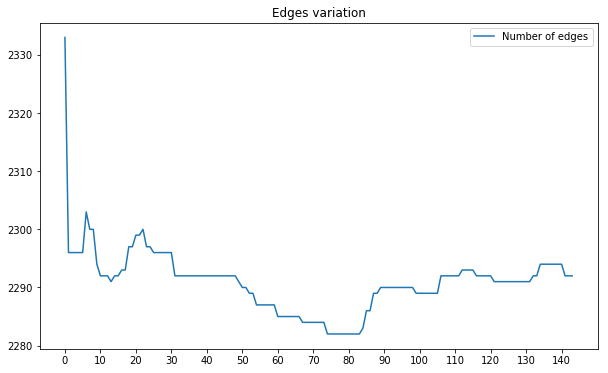
\includegraphics[width=\linewidth]{daily_number_of_edges0}
			\caption{Snapshot, May 16th}
			\label{daily_edges0}
		\end{subfigure}
		\begin{subfigure}{0.45\textwidth}
			\centering
			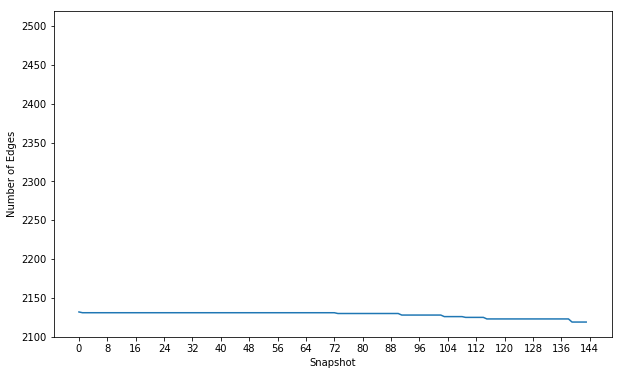
\includegraphics[width=\linewidth]{daily_number_of_edges1}
			\caption{Snapshot, May 21th}
			\label{daily_edges1}
		\end{subfigure}
		\begin{subfigure}{0.45\textwidth}
			\centering
			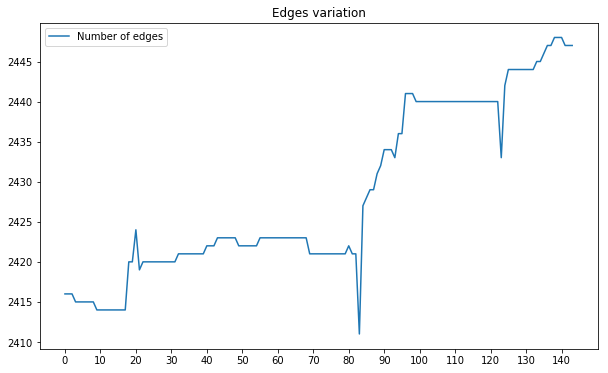
\includegraphics[width=\linewidth]{daily_number_of_edges2}
			\caption{Snapshot, May 26th}
			\label{daily_edges2}
		\end{subfigure}
		\begin{subfigure}{0.45\textwidth}
			\centering
			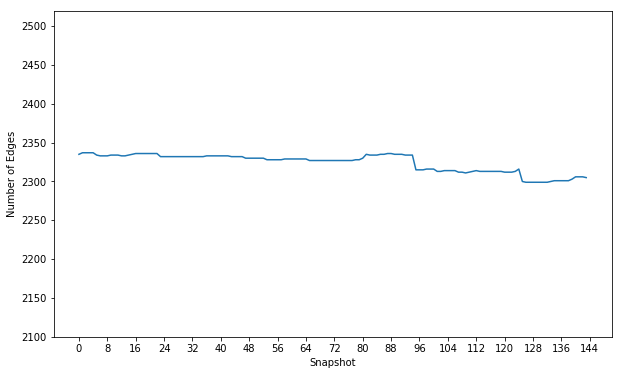
\includegraphics[width=\linewidth]{daily_number_of_edges3}
			\caption{Snapshot, June 2nd}
			\label{daily_edges3}
		\end{subfigure}
		
		\caption{Edges trends on a daily basis}
		\label{daily_edges_variation}
	\end{figure}

	The trends for edges essentially follow the same behavior of the node. It is trivial to see that for each node connecting (disconnecting) to the network, at least one channel is added (removed). The actual number of edges per node will be shown in the next section.
	
	\begin{center}
	\begin{tabulary}{\linewidth}{| L | C | C | C | C |}
		\hline
		& May 16th (\ref{daily_edges0}) & May 21th (\ref{daily_edges1}) & May 26th (\ref{daily_edges0}) & June 2nd (\ref{daily_edges3}) \\
		\hline
		Starting edges & 2333 & 2132 & 2416 & 2335 \\ \hline
		Final edges & 2292 & 2119 & 2447 & 2305 \\ \hline
		Variation(\%) & -1.75\% & -0.60\% & +1.28\% & -1.28\% \\ \hline
		Max num. edges & 2333 & 2132 & 2448 & 2337 \\ \hline
		Min num. edges & 2282 & 2119 & 2411 & 2299 \\ \hline	
	\end{tabulary}
	\end{center}

	\newpage
	\subsection{Daily average degree variation}

		

	\begin{figure}[t]
		\centering
		\begin{subfigure}{0.45\textwidth}
			\centering
			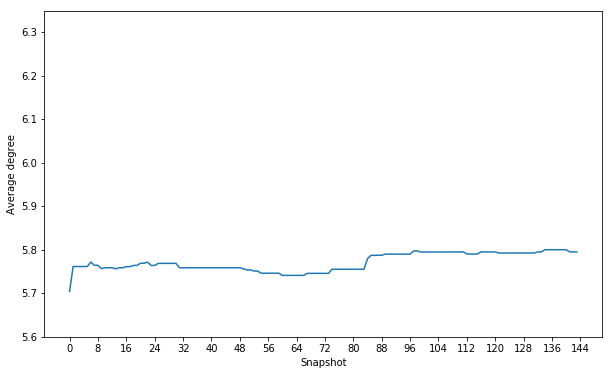
\includegraphics[width=\linewidth]{daily_average_degree0}
			\caption{Snapshot, May 16th}
			\label{daily_degree0}
		\end{subfigure}
		\begin{subfigure}{0.45\textwidth}
			\centering
			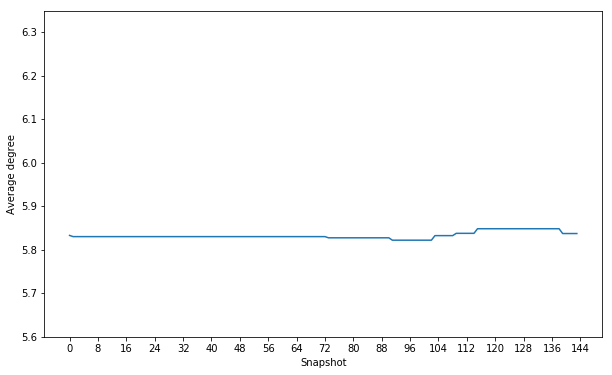
\includegraphics[width=\linewidth]{daily_average_degree1}
			\caption{Snapshot, May 21th}
			\label{daily_degree1}
		\end{subfigure}
		\begin{subfigure}{0.45\textwidth}
			\centering
			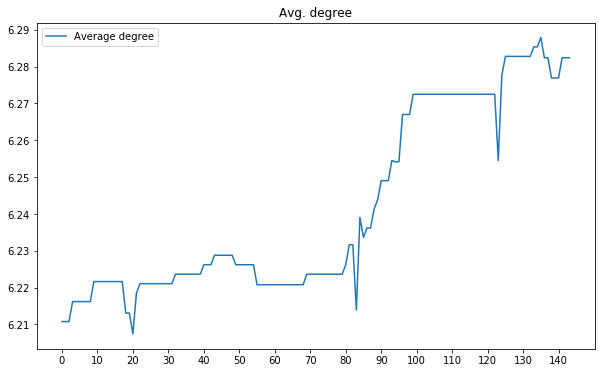
\includegraphics[width=\linewidth]{daily_average_degree2}
			\caption{Snapshot, May 26th}
			\label{daily_degree2}
		\end{subfigure}
		\begin{subfigure}{0.45\textwidth}
			\centering
			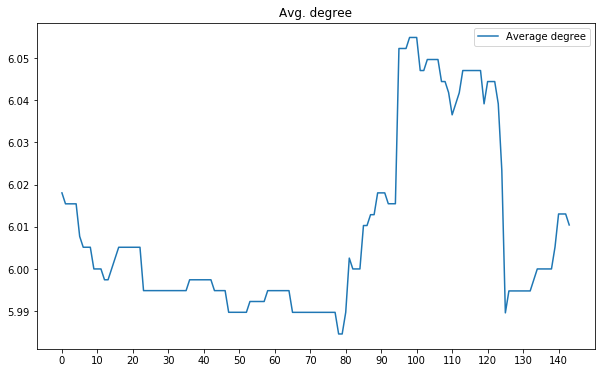
\includegraphics[width=\linewidth]{daily_average_degree3}
			\caption{Snapshot, June 2nd}
			\label{daily_degree3}
		\end{subfigure}
		
		\caption{Average degree on a daily basis}
		\label{daily_degree _variation}
	\end{figure}
		\begin{center}
		\begin{tabulary}{\linewidth}{| L | C | C | C | C |}
			\hline	
			& May 16th (\ref{daily_degree0}) & May 21th (\ref{daily_degree1}) & May 26th (\ref{daily_degree2}) & June 2nd (\ref{daily_degree3}) \\
			\hline
			Starting degree & 5.70 & 5.833 & 6.21  & 6.018 \\ \hline
			Final degree & 5.79 & 5.837 & 6.28 & 6.010 \\ \hline
			variation & +1.59\% & +0.07\% & +1.15\% & -0.12\% \\ \hline
			Max avg. degree & 5.80 & 5.84 & 6.28 & 6.05 \\ \hline
			Min avg. degree & 5.70 & 5.82 & 6.20 & 5.98 \\ \hline		
		\end{tabulary}
	\end{center}
	
	\subsection{Daily diameter}
	\subsection{Daily average eccentricity}
	\subsection{Weekly nodes variation}
	\subsection{Weekly edges variation}
	\subsection{Weekly average degree variation}
	\subsection{Weekly diameter}
	\subsection{Weekly average eccentricity}
	\section{Betwenness	 centrality}
	\subsection{Daily betweenness centrality - top 5}
	\subsection{Gantt chart - day}
	\subsection{Weekly betweenness centrality - top 5}
	\subsection{Gantt chart - week}
	\section{\textit{k}-vertex connectivity}
	\subsection{Components size}
	\subsection{Betweenness inclusion}
	\section{Max-Cut}
\end{document}